\section{Methods for monocular reconstruction of articulated subjects}

Having now discussed methods for modelling articulated subjects, the next topic for consideration is how to incorporate such models in 3D reconstruction pipelines. In general, the methods listed take as input an image or video sequence $I_{1 \dots N}$ depicting a subject, and output a set of 3D model parameters $\alpha$ (often factored into shape $\shape$ and $\pose$). These parameters can then supplied to the model's correponding generator function $g: \alpha \mapsto \R{3}$ (e.g. $\SMPL(\shape, \pose)$ or $\SMAL(\shape, \pose)$) in order to obtain the 3D model prediction $v \in \R{3}$. 

Methods which attempt to align a parametric 3D model to a single image dates back as far as 1963, in a seminal paper presented by Roberts~\cite{xxx}. In this work, viewpoint and cuboidal block parameters were predicted to fit a 2D line image. Model-based methods were also applied to understand object structure captured in 2D images, beginning with geometric primitives~\cite{xxx} to Active Shape Models, which use a training data set to learn priors over a designed deformable model. These techniques inspired the work of Blanz and Vetter~\cite{blanz-vetter} who built the first 3D morphable face model by aligning 3D scans and optimized the parameters to provide a fit to a single image. We will leave further discussion on reconstructing faces and hands to the following survey papers~\cite{xxx, xxx}, and focus instead on reconstructing the full human body and animals.

It is important to note that all classes of approaches must overcome significant ambiguity. Determining joint positions is a task made challenging due to large variations in visual appearence, commonly due to clothing, body shape and camera view. As explained by Toshev and Szegedy~\cite{toshev2014deeppose}, even with perfect joint locations the subsequent lifting step is also ill-posed, as the space of consistent 3D poses for given 2D landmark locations is infinite. This is typically resolved using strong prior knowledge which usually takes the form of 3D geometric pose priors and temporal or structural constraints.

\subsection{3D Pose Estimation}

    The first class of techniques, known as methods for 3D pose estimation output a set of 3D keypoint locations which can be combined to form a skeleton. Since only a skeleton outline is obtained, apart from basic limb measurements, no other shape detail (e.g. surface definition, object density etc.) is obtained. However, it should be noted that this output form is often perfectly satisfactory depending on the intended application. In particular, this family of techniques have found numerous applications in controllerless gaming (e.g. Microsoft Kinect~\cite{kinectpaper}), motion capture (e.g. for digital character generation~\cite{xxx}), gait analysis (e.g. identifying lameness in cattle~\cite{xxx}) and many more. 

    Early approaches in this category built human stick figures with various constrained including assumptions of fixed limb lengths{xxx}, length ratios~\cite{xxx} or that limb lengths are isometric across individuals and vary only in global scaling~\cite{xxx}. More advanced techniques built statistical models of shape variation using anthropometric tables or learnt statistical models from freely available motion capture data~\cite{barron2001estimating}. The idea then is to fit such a model to each frame of an input image or video sequence. 

    A notable early work in this category is that of Shotton et al.~\cite{kinectpaper} (see~\cref{fig:kinect_skeleton}) who designed a commercially available human skeletal tracking capability, albeit one that requires a depth sensor at test time. Their technique employed a generative 3D human body model to synthesize a large training dataset of depth images with corresponding body part labels. Density estimators for each body part are then used in combination to localize body joints with a calculated confidence value. Chapter 3 of this thesis demonstrates a technique for predicting keypoints by training on synthetic silhouette data rendered from an animal deformable body model.

    More recent approaches typically employ a 2-stage pipeline; they begin by localizing 2D joint positions on an input image before running a subsequent optimization step that `lifts` these to a 3D pose.  Examples of such systems include DeepPose~\cite{toshev2014deeppose}, an approach which employs a CNN to reason jointly about 2D landmark detection and 3D pose estimation from single RGB images. Pishchulin et al.~\cite{pishchulin2016deepcut} later introduced DeepCut which extends DeepPose to the multi-person case. Both systems are trained on large body joint databases. 

    
    \begin{figure}[H] % Example image
        \center{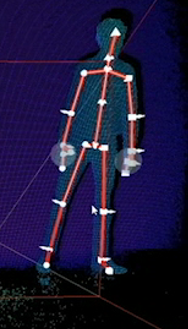
\includegraphics[width=0.25\linewidth]{human_tracking}}
        \caption{Kinect generating per-pixel joint proposals.}
        \label{fig:kinect_skeleton}
    \end{figure}

    \subsection{Multi-stage approaches}
    

    \subsection{Direct approaches}
    However, some direct techniques exist which do not require an initial 2D joint prediction. These include methods that directly regress to a 3D pose~\cite{tekin2016direct}. However, these typically rely on an annotated set of 3D joint labels, which can be difficult and costly to obtain, or being able to build a representative synthetic dataset, which is non-trivial task.


\subsection{Toolkit}

\subsubsection{Rendering}
    The process of generating a 2D image from a 3D polygon mesh is known as rendering and can be achieved through a process known as raytracing. Raytracing is a rendering technique able to generate photorealistic 2D images from the scene. It can be considered the opposite process by which the human eye perceives the world, as this method involves lines being cast outwards, beginning at a point known as the \emph{camera origin}. Figure \ref{fig:raycasting} shows a typical set up, in which rays are cast from the camera origin through each pixel on the image plane. The colour for the pixel is obtained by following the ray through the scene until a light source or non-reflective surface is reached, taking into account any reflections or non-opaque scene items. Due to the considerable comptuation required, the operation is often parallelized and assigned to the GPU. However, the technique is typically considered unsuitable for real-time rendering of complex scenes (due to complex ray paths) or when high resolution images (many rays required) are needed. However, for this work, scenes are typically made up of a single non-reflective, solid mesh surface and contain no complex elements (e.g.\ shadows, non-constant lighting.

    \begin{figure}[H] % Example image
        \center{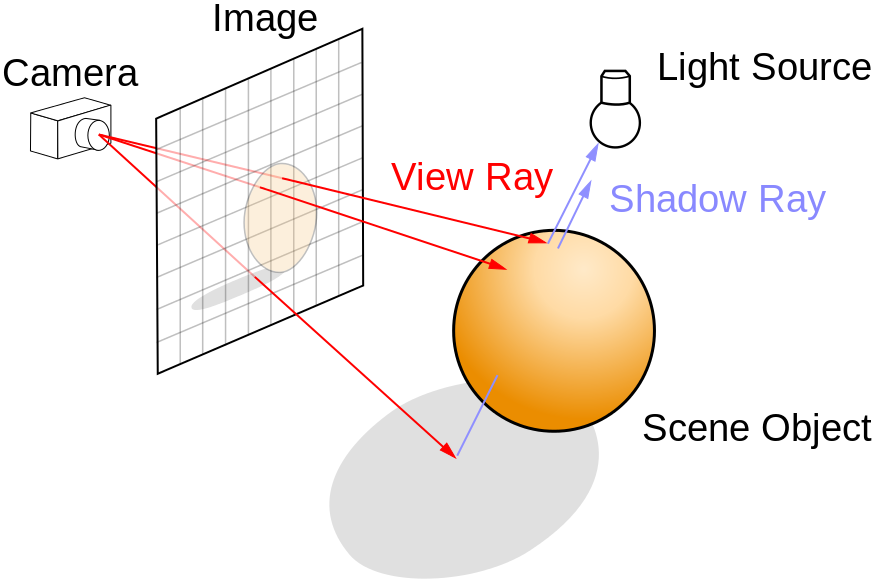
\includegraphics[width=0.5\linewidth]{ray_trace}}
        \caption{Diagram showing raycast rendering.~\cite{rendering}.}
        \label{fig:raycasting}
    \end{figure}

    It is also worth noting that the standard method for raycasting is not differentiable, causing problems for differentiable optimizers (including neural networks). However, alternative rendering methods~\cite{loper2014opendr} are available for these purposes.

\subsubsection{Model fitting: fitting a template model to correspondences}
    % Edit to talk about e.g. SMPLify

    %  Model fitting algorithms are typically provided with point correspondences between the template mesh and input images in order to help constrain the optimization. Correspondences are either provided by a human annotator or predicted by a discriminative machine learning model.

    Taylor et al. demonstrate a model fitting approach that operates on a rigged 3D human mesh~\cite{taylor2012vitruvian}. Their aim is to learn a set of pose parameters $\theta \in \mathbb{R}^{d}$ so as to explain a set of image points $D = \{x_{i}\}_{i=0}^{n}$. Data points $x_{i} \in \mathbb{R}^{3}$ are collected from a calibrated depth camera. Once these pose parameters are learnt, the mesh is deformed according to the LBS algorithm defined above.

    The template mesh contains $|J| = 13$ joints, and $m$ skinned vertices ${V} = \{v_{i}\}_{i=1}^{m}$. Again, each vertex $v_{i} \in V$ is defined as:

    \begin{equation}
        v_{i} = (x_{i}, s_{i})
    \end{equation}
    where $x_{i} \in \mathbb{R}^{3}$ represents the base 3D vertex positions in a canonical pose $\theta_{0}$ and the $s_{i} \in \mathbb{R}^{|J|}$ are skinning weight vectors. It is possible to define a mesh induced by a pose $S(\theta) = (V, T)$ for vertices $V$ and triangles $T$. Due to the resemblance of the mesh surface induced by the canonical mesh pose $\theta_{0}$ and Da Vinci's Vitruvian man~\cite{davinci}, this surface is referred to as the \emph{Vitruvian Manifold}, and is shown in Figure~\ref{fig:vitruvian_man}. 

    \begin{figure}[H] % Example image
        \center{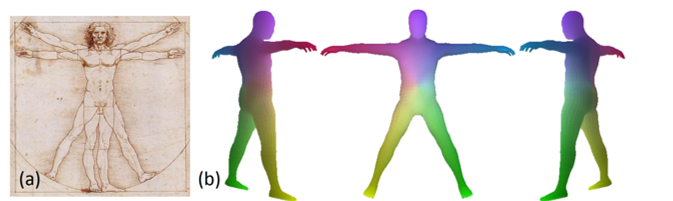
\includegraphics[width=0.95\linewidth]{vitruvian_man}}
        \caption{(a) Vitruvian Man by Leonardo da Vinci~\cite{davinci} and (b) the Vitruvian Manifold reprinted from~\cite{taylor2012vitruvian}.}
        \label{fig:vitruvian_man}
    \end{figure}

    The primary contribution of this paper is the design of a model able to predict \emph{dense correspondences} between the 3D canonical mesh and input 3D images. In other words, \emph{every} body pixel on an input image is regressed to a point on the vitruvian manifold mesh. The authors demonstrate the accuracy of these correspondences is sufficient for \emph{one-shot learning}, meaning there is no need to recalculate correspondences after a subsequent optimization step. The reason for this is the strength of the core error term which penalizes the sum of errors between image points $\{x_{i}\}_{i=0}^{n}$ and determined mesh correspondences $U = \{u_{i}\}_{i=0}^{n} \subseteq V$:

    \begin{equation}
        E_{\text{data}}(\theta,U) =\sum_{i=1}^{n}s_{i} \cdot d(x_{i}, M(u_{i}; \theta))
    \end{equation}
    where $M(u_{i}, \theta)$ is the position of vertex $u_{i}$ on the vitruvian manifold mesh after having been displaced by an LBS deformation with respect to the pose~$\theta$. 

    The sheer quantity of correspondences greatly constrain their optimizer which works well, even on challenging input images. Much of this report focuses on how this paper can be extended to work for animal subjects, incorporating deep learning correspondence prediction and working from monocular RGB input data.

\subsubsection{Model parameter regression}

    This is how you do this using a deep network. 


\subsection{Model-based faces and hands}


\begin{figure}[H] % Example image
    \center{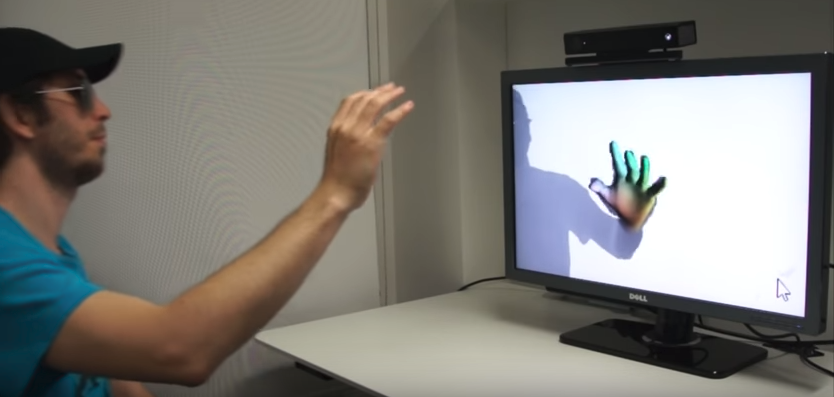
\includegraphics[width=0.85\linewidth]{hand_tracking}}
    \caption{Example of articulated hand tracking, reprinted from~\cite{taylor2016efficient}.}
    \label{fig:hand_tracking}
\end{figure}


\subsection{Model-based human shape and pose}

% only discuss dense methods -- discuss methods that do/do not explicitly model shape

The majority of recent work in 3D pose and shape recovery from monocular images tackles the special case of 3D \emph{human} reconstruction. As a result, the research community has collected a multitude of open source human datasets which provide strong supervisory signals for training deep neural networks. These include accurate 3D deformable template models~\cite{loper15smpl} generated from real human scans, 3D motion capture datasets~\cite{ionescu2013human3,vonmarcard2018recovering} and large 2D datasets~\cite{lin2014microsoft,johnson2010clustered,andriluka14cvpr} which provide keypoint and silhouette annotations. 

The abundance of available human data has supported the development of successful monocular 3D reconstruction pipelines~\cite{kolotouros19convolutional,kanazawa18end-to-end}. Such approaches rely on accurate 3D data to build detailed priors over the distribution of human shapes and poses, and use large 2D keypoints datasets to promote generalization to ``in-the-wild'' scenarios. Silhouette data has also been shown to assist in accurate reconstruction of clothes, hair and other appearance detail~\cite{pifuSHNMKL19,alldieck2019learning}.
While the dominant paradigm in human reconstruction is now end-to-end deep learning methods, SPIN~\cite{kolotouros19learning} show impressive improvement by incorporating an energy minimization process within their training loop to further minimize a 2D reprojection loss subject to fixed pose \& shape priors. Inspired by this innovation, we learn an iteratively-improving shape prior by applying expectation maximization 
during the training process.

\subsubsection{Fitting the SMPL mesh to human images}
SMPLify \cite{bogo16keep} is a fully-automated optimization approach that uses predicted human joint positions to constrain a optimizer that fits the aforementioned SMPL model to RGB input images. It first makes use of the DeepCut CNN to predict 2D human body joints $J_{\text{est}}$ on input frames. For each 2D joint $i$ the CNN is able to provide a confidence value $w_i$ for the joint's position. The optimization begins by first solving for global rotation (i.e. $\theta_{0..2}$) and global translation $\gamma$ by fitting a small number of 2D torso points $J_{\text{torso}} \subset J_{\text{est}}$ to the data. The user is expected to provide a value for the focal length $f$. Then, the full optimization takes place, fitting 3D pose and shape to all 2D joints by minimizing the following objective function which comprises five error terms:

\begin{equation}
E(\beta, \theta) = E_{J}(\beta, \theta; K, J_{\text{est}}) + \lambda_{\theta}E_{\theta}(\theta) + \lambda_{\alpha}E_{\alpha}(\theta) + \lambda_{\text{sp}}E_{\text{sp}}(\theta; \beta) + \lambda_{\beta}E_{\beta}(\beta)
\end{equation}
where $\lambda$ terms are the scalar weights. The term $E_{J}$ is often referred to as the \textit{data} term, as it places most emphasis on constraining the model to the input sensory data. The job of this term is to penalize the weighted 2D distance between estimated joints $J_{\text{est}}$ and corresponding projected SMPL joints. In practice, this projection takes place using the OpenDR differentiable rendering framework to ensure the final formulation remains differentiable:

\begin{equation}
    E_{J}(\beta, \theta; K, J_{\text{est}}) = \sum_{joint j} w_{j} \rho(\Pi_{K}(R_{\theta}(J(\beta)_j)) - J_{\text{est}, j})
\end{equation}
where $J(\beta)$ is a function which predicts 3D body joints from body shape and $R_{\theta}(J(\beta))$ therefore denote posed 3D joints.

The remaining terms are now briefly discussed:
\clearpage
\begin{itemize}
    \item $E_{\theta}(\theta)$ is referred to as a \textit{pose prior} which favours more likely poses by assigning large punishment to those that deviate from known poses collected from a large dataset.
    \item $E_{\beta}(\beta)$ is referred to as a \textit{shape prior} which favours more likely pose-invariant shape configurations by assigning large punishment to those that deviate from known shapes collected from a large dataset. 
    \item $E_{\alpha}(\theta)$ is a \textit{joint limit} prior which ensures particular joints remain within acceptable angle limits. For example, a knee joint in a human model should be prohibited from bending more than 5 degrees upwards.
    \item $E_{sp}(\theta; \beta)$ is an \textit{interpenetration} term, which can only be defined in such shape modelling approaches. Using both shape and pose from the model, it is possible to determine if any limbs are self-intersecting, or intersect other parts of the body and assign appropriate penalty.
\end{itemize}

An example result can be seen in Figure \ref{fig:smplify}:

\begin{figure}[H] % Example image
    \center{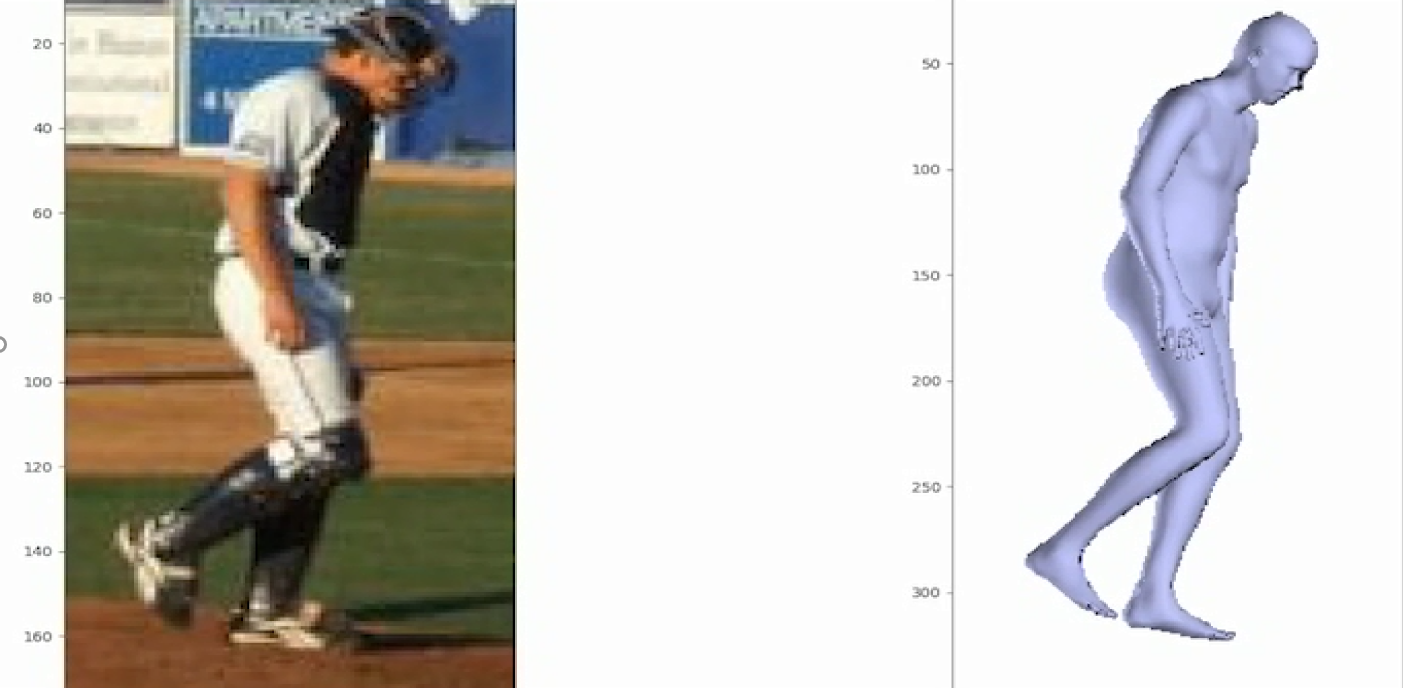
\includegraphics[width=0.95\linewidth]{fitting_smpl}}
    \caption{SMPLify: Fitting the SMPL model to the Leeds Sports Dataset.}
    \label{fig:smplify}
\end{figure}
        
\subsection{Direct regression}
The most recent, and state-of-the-art approaches employ deep learning techniques to solve the entire optimization problem by directly regressing to shape and pose parameters of the template model. Tekin et al.~\cite{tekin2016direct} introduce a convolutional network trained on the Human3.6m dataset~\cite{lin2014microsoft} that directly regresses to a human pose defined in terms 3D locations $y \in \mathbb{R}^{3J}$ of $J$ body joints relative to a root joint. Tan et al.~\cite{tan17indirect} introduce an approach that directly regresses to SMPL parameters from synthetic images, ensuring suitable image jitters are applied to promote generality to real-world images. The method is termed Indirect Learning, and is trained from real human images with no known corresponding SMPL parameters. An autoencoder network is introduced, and a decoder first trained from synthetic (SMPL parameter, rendered image) pairs to construct an automatic renderer. This part of the network is then frozen, before the entire autoencoder is trained on many segmented human images that optimize the encoder to real-world examples. The end result is a process that is able to predict SMPL parameters from real-world human images. An example result is shown in Figure~\ref{fig:indirect_learning}.

\begin{figure}[H] % Example image
    \center{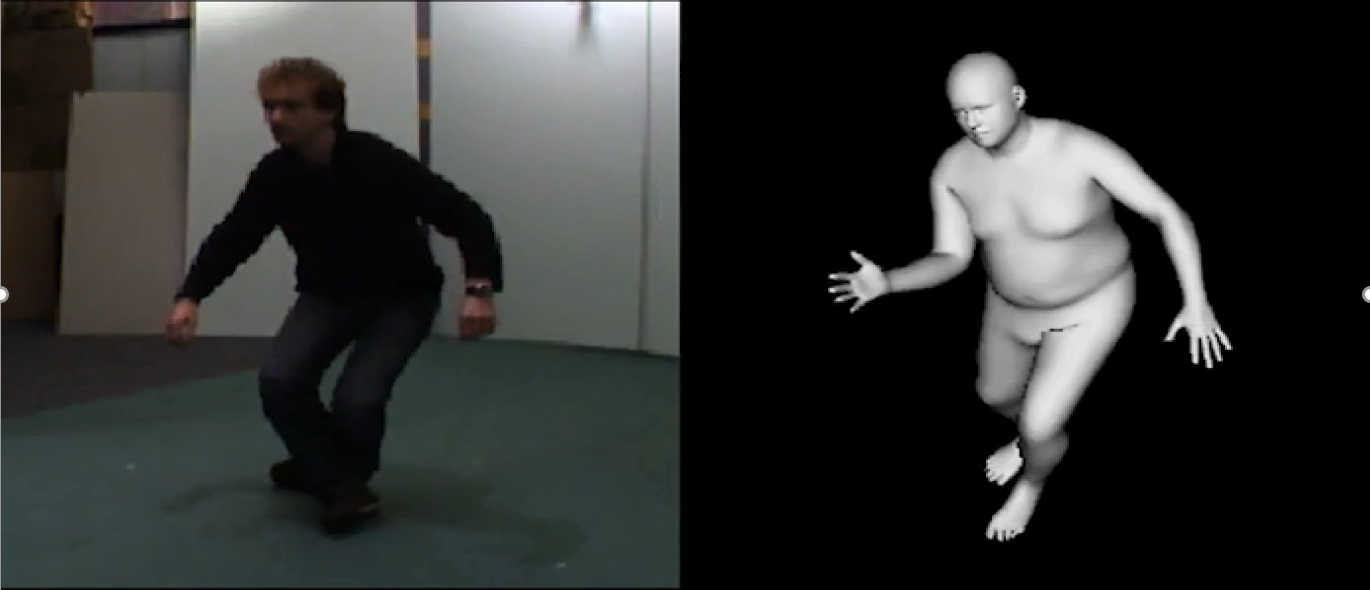
\includegraphics[width=0.75\linewidth]{indirect_learning}}
    \caption{Indirect learning method regressing to SMPL parameters from an RGB video sequence. Reprinted from~\cite{tan17indirect}.}
    \label{fig:indirect_learning}
\end{figure}


\subsection{Model-based animals}

We want to do model based reconstruction to impose a prior on the fitting and also automatically recover an interpretable fit.

\subsubsection{Animals intro}

Cashman and Fitzgibbon~\cite{cashman2013shape} obtained one of the first 3D morphable animal models, but their work was limited to small classes of objects (e.g. dolphins, pigeons), and did not incorporate a skeleton.  Their work also showed the use of the 2D silhouette for fitting, which is key to our method. 
Reinert {\em et al.} \cite{reinert2016animated} meanwhile construct 3D meshes by fitting generalized cylinders to hand-drawn skeletons.
Combined skeletal and morphable models were used by Khamis {\em et al.}~\cite{hand-shape} for modelling the human hand, and Loper {\em et al.}~\cite{loper15smpl} in the SMPL model which has been extensively used for human tracking. 

The SMPL model was extended to animals by Zuffi {\em et al.}~\cite{zuffi2017menagerie}, where the lack of motion capture data for animal subjects is cleverly overcome by building the model from $41$ 3D scans of toy figurines from five quadruped families in arbitrary poses. Their paper demonstrates single-frame fits of their model to real-world animal data, showing that despite the model being built from ``artists' impressions'' it remains an accurate model of real animals. This is borne out further by our work.  Their paper did however depend on per-frame human annotated keypoint labels, which would be costly and challenging to obtain for large video sequences. This work was recently extended~\cite{zuffi_lions} with a refinement step that optimizes over model vertex positions. This can be considered independent to the initial SMAL model fit and would be trivial to add to our method.


\subsubsection{Fitting to animal video sequences}

While animals are often featured in computer vision literature, there are still relatively few works that focus on accurate 3D animal reconstruction. 

A primary reason for this is the lack of large scale 3D datasets stemming from the practical challenges associated with 3D motion capture, as well as a lack of 2D data which captures a wide variety of animals. The recent Animal Pose dataset~\cite{animalpose} is one such 2D alternative, but contains significantly fewer labelled images than our new StanfordDogs dataset (4,000 compared to 20,580 in ). 
On the other hand, animal silhouette data is plentiful~\cite{lin2014microsoft,everingham2010pascal,DAVIS2017-2nd}.

Zuffi et al.~\cite{zuffi2017menagerie} made a significant contribution to 3D animal reconstruction research by releasing SMAL, a deformable 3D quadruped model (analagous to SMPL~\cite{loper15smpl} for human reconstruction) from $41$ scans of artist-designed toy figurines. The authors also released shape and pose priors generated from artist data. In this work we develop \emph{SMBLD}, an extension of SMAL that better represents the diverse dog category by adding scale parameters and refining the shape prior using our large image dataset.

While there have been various ``model-free'' approaches which do not rely on an initial template model to generate the 3D animal reconstruction, these techniques often do not produce a mesh~\cite{Agudo_2018_CVPR,novotny19c3dpo} or rely heavily on input 2D keypoints or video at test-time~\cite{vicente_3dv,Probst2018_ECCVa}. An exception is the end-to-end network of Kanazawa et al.~\cite{kanazawa2018birds}, although we argue that the bird category exhibits more limited articulation than our dog category.

We instead focus on model-based approaches. The SMAL authors~\cite{zuffi2017menagerie} demonstrate fitting their deformable 3D model to quadruped species using user-provided keypoint and silhouette dataset. SMALR~\cite{zuffi_lions} then demonstrated fitting to broader animal categories by incorporating multi-view constraints from video sequences. Biggs et al.~\cite{biggs2018creatures} overcame the need for hand-clicked keypoints by training a joint predictor on synthetic data. 3D-Safari~\cite{Zuffi19Safari} further improve by training a deep network on synthetic data (built using SMALR~\cite{zuffi_lions}) to recover detailed zebra shapes in the wild.

A drawback of these approaches is their reliance on a test-time energy-based optimization procedure, which is susceptible to failure with poor quality keypoint/silhouette predictions and increases the computational burden. By contrast our method requires no additional energy-based refinement, and is trained purely from single in-the-wild images. The experimental section of this paper contains a robust comparison between our end-to-end method and relevant optimization-based approaches. 


A major impediment to research in 3D animal reconstruction has been the lack of a strong evaluation benchmark, with most of the above methods showing only qualitative evaluations or providing quantitative results on fewer than 50 examples. To remedy this, we introduce \emph{StanfordExtra}, a new large-scale dataset which we hope will drive further progress in the field. 


Stebbing et al.~\cite{arap_stebbing} introduce a technique capable of fitting a template mesh to live video sequences for a range of different animal species. Some user interaction is required in order to segment the animal from the background and to provide sparse 3D-mesh-to-2D-image key point correspondences. This work only operates on input video sequences (rather than single frames), so a number of temporal terms are incorporated that encourage sensible inter-frame model deviation. The system requires an annotated input template mesh representative of the target animal species. Note that this work does not require the template mesh to have an inner skeletal structure. However, the user assists an ARAP-style term by assigning each mesh vertex $v_i$ to one of $M$ groups which share a set of basis rotations $B_{m}$. 

\begin{figure}[H]
    \centering
    \begin{subfigure}{0.5\textwidth}
    \centering
        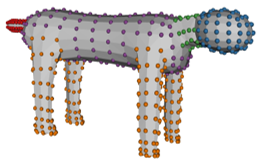
\includegraphics[height=0.5\linewidth]{arapsfm/arap_annotated_template}
        \caption{Template mesh with joint movement constraints.}
    \end{subfigure}%
    \begin{subfigure}{0.5\textwidth}
    \centering
        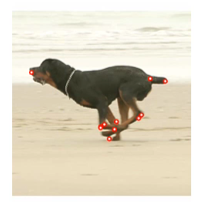
\includegraphics[height=0.5\linewidth]{arapsfm/arap_point_tracks}
        \caption{Example of user supplied point tracks.}
    \end{subfigure}%
    \caption{User input required for the deformable mesh animation algorithm, reprinted from~\cite{arap_stebbing}.}
    \label{fig:arap_user}
\end{figure} 

Through reasonably accurate pose fitting and by allowing some pose-invariant shape deformation, this work produces smooth meshes which are often a good match to the input video. Moreover, their experimentation shows that ARAP is a useful prior for reconstructing articulated, non-rigid motion in instances that an internal skeleton is a priori unknown. However, the shape attributes for the reconstructed model are not particularly accurate, which results in frequent errors appearing at internal occluding contours. In addition, the large non-convex optimization algorithm is an expensive operation, taking around 1 minute per video frame on a standard Linux workstation.

Results showing this work fitting a crude dog template mesh to a sample video obtained from YouTube are shown previously in Figure \ref{fig:intro_arap_output}. Figure \ref{fig:arap_output} shows another example, which operates on a template impala mesh.

\begin{figure}[H]
    \center{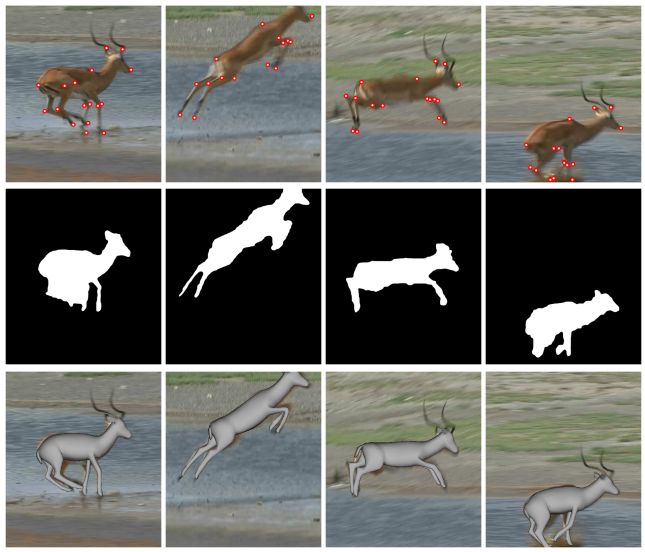
\includegraphics[width=0.95\linewidth]{arapsfm/arap_impala}}
    \caption{Example of an impala template being fit to input video sequence, reprinted from~\cite{arap_stebbing}}
    \label{fig:arap_output}
\end{figure}

\subsubsection{Learning animal shape from unrelated 2D images}
Cashman and Fitzgibbon~\cite{cashman2013shape} introduce an optimization technique able to recover a parameterized, morphable 3D model from unrelated 2D images depicting examples of the target class. The method requires user-supplied 2D object outlines and point constraints for each image, and a single rigid mesh for the entire object class. The authors demonstrate recovering an 8-parameter morphable dolphin model from 32 images obtained from Google. To reduce required user activity, it is reasonable to assume that given sufficient labelled training data, it would be simple to manipulate a convolutional network architecture able to perform foreground / background segmentation and identify human key points (say, joints) for the desired object class. The system achieves impressive results when optimizing over both pose and shape parameters across a range of object classes, but struggles for articulated models such as polar bears.

\begin{figure}[H] % Example image
    \center{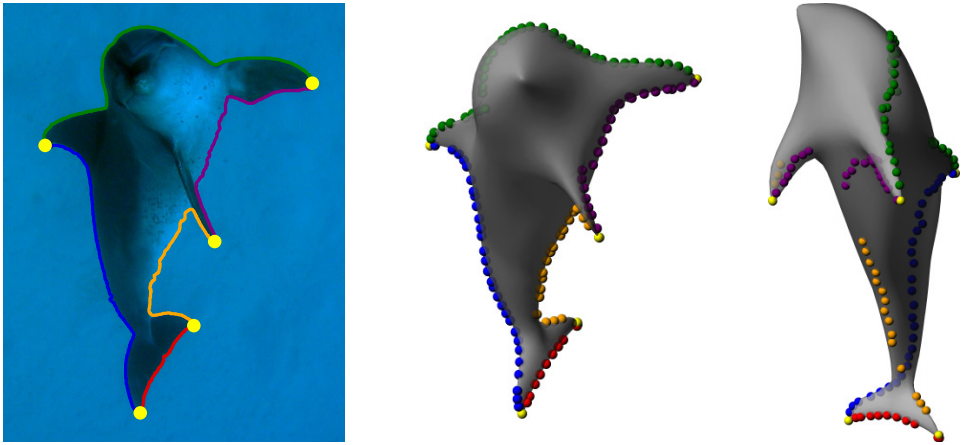
\includegraphics[width=0.7\linewidth]{dolphins}}
    \caption{8-parameter dolphin model with annotated contour (left) and contour generators (middle and right).}
    \label{fig:cashman_fitzgibbon}
\end{figure}

\subsubsection{Fitting the SMAL mesh to animal images}
The SMAL paper briefly discusses a modification to the SMPLify approach in order to fit the SMAL model to RGB animal input images. The terms are largely the same, although the interpenetration term is omitted and joint positions are provided manually, rather than being predicted by a CNN. Finally, the optimizer requires a pre-segmented (i.e.\ silhouette) image which is also supplied by a user. An approach discussed in Chapter 4 builds on this work, so an in-depth description of this method is ommited here. However, an example result showing the result of the optimizer fitting the SMAL mesh to an RGB image of a fox can be seen in Figure \ref{fig:smalify}. Note that the whole optimization process takes around 1 minute per frame.

\begin{figure}[H] % Example image
    \center{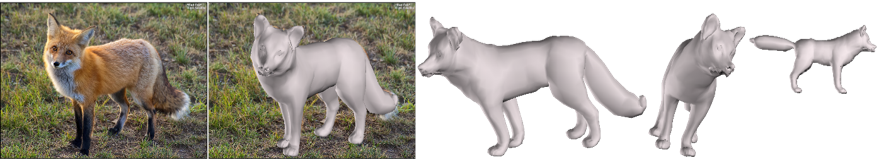
\includegraphics[width=0.95\linewidth]{fitting_smal}}
    \caption{Fitting SMAL to a hand segmented animal, reprinted from~\cite{zuffi2017menagerie}.}
    \label{fig:smalify}
\end{figure}

\subsubsection{Literature review tables}

The closest work in terms of scale is the category-specific mesh reconstruction of Kanazawa et al.~\cite{kanazawa2018birds}, where 2850 images of birds were reconstructed.  However doing so for the complex pose and shape variations of dogs required the advances described in this paper.

Table~\ref{tab:literature} summarizes previous work on animal reconstruction.
It is interesting to note that while several papers demonstrate reconstruction across species, which {\em prima facie} is a richer class than just dogs, the test-time requirements (e.g. manually-clicked keypoints/silhouette segmentations, input image quality etc.) are considerably higher for those systems.
Thus we claim that the achievement of reconstructing a full range of dog breeds, 
with variable fur length, varying shape and pose of ears, and with considerable occlusion, is a significant contribution.


